\chapter{Stationary black holes}
\label{s:sta}\index{stationary!black hole}

\minitoc

\section{Introduction}

This chapter is still in draft stage...

\section{Definition and first properties}

\subsection{Stationarity and staticity} \label{s:sta:def_station}

Let us start by defining the concepts of \emph{stationary} and \emph{static}
spacetimes.

\begin{greybox}
A spacetime $(\M,\w{g})$ is called \defin{stationary}\index{stationary!spacetime}
iff (i) it is invariant under
the action of the translation group $(\mathbb{R},+)$ and (ii) the orbits of
the group action (cf. Sec.~\ref{s:neh:symmetries})
are everywhere timelike curves or (ii') $(\M,\w{g})$
admits a conformal completion (cf. Sec.~\ref{s:glo:conf_compl})
and the orbits of the group action are timelike in the vicinity of
the conformal boundary $\scri$.
It is equivalent to say that there exists a Killing vector field
$\w{\xi}$ (the generator of the translation group, cf. Sec.~\ref{s:neh:symmetries}) that is
timelike everywhere or at least in the vicinity of $\scri$ when there exists a conformal
completion. We shall say that $(\M,\w{g})$ is \defin{strictly stationary}\index{strictly!stationary}\index{stationary!strictly --} iff the Killing vector field $\w{\xi}$ is timelike in all $\M$,
i.e. iff the point (ii) above is fulfilled.
\end{greybox}

\begin{remark} \label{r:sta:pseudo-stationary}
Some authors (e.g. Carter \cite{Carte73b}) call
\emph{pseudo-stationary}\index{pseudo-stationary} the stationary spacetimes
defined above, keeping the qualifier
\emph{stationary} for the strictly stationary case.
As we are going to see, when $\M$
contains a black hole, $\w{\xi}$ cannot be timelike everywhere,
so only \emph{pseudo-stationarity} in the above sense is relevant for these spacetimes.
Our terminology follows that of
Heusler \cite{Heusle96},
Chru\'sciel, Lopes Costa \& Heusler \cite{ChrusLH12}
and Choquet-Bruhat \cite{Choqu09}.
\end{remark}

A notion stronger than stationarity is that of \emph{staticity}:

\begin{greybox}
A spacetime $(\M,\w{g})$ is called \defin{static}\index{static!spacetime}
iff (i) it is stationary and (ii) the Killing vector field $\w{\xi}$
generating the stationary action is orthogonal to a family of hypersurfaces
(one says that $\w{\xi}$ is \defin{hypersurface-orthogonal}\index{hypersurface-orthogonal}).
The spacetime $(\M,\w{g})$ is called \defin{strictly static}\index{strictly!static}\index{static!strictly --}
iff $\w{\xi}$ is timelike in all $\M$.
\end{greybox}

\begin{remark}
The same comment as in Remark~\ref{r:sta:pseudo-stationary} can be made: some authors
would call \emph{static} only spacetimes that are
\emph{strictly static} according to the above definition.
\end{remark}

Via the Frobenius theorem (cf. Sec.~\ref{s:def:Frobenius}), the hypersurface-orthogonal
condition is equivalent to the existence of a 1-form $\w{\omega}$ such that
\be \label{e:sta:dxi_Frob}
    \dd \uu{\xi} = \w{\omega} \wedge \uu{\xi} ,
\ee
where $\uu{\xi}$ is the metric dual of $\w{\xi}$ (cf. Sec.~\ref{s:bas:metric_dual}).
Equation (\ref{e:sta:dxi_Frob}) is equivalent to
\be
    \uu{\xi}\wedge\dd\uu{\xi} = 0 ,
\ee
or, in terms of components (expressing the exterior derivative $\dd\uu{\xi}$ in
terms of the spacetime Levi-Civita connection $\wnab$):
\be
    \xi_{[\alpha} \nabla_\beta \xi_{\gamma]} = 0.
\ee
Then, one can show (see e.g. Sec.~2.9 of Straumann's textbook \cite{Strau13}), that locally, there exists a coordinate system $(x^\alpha)=(t,x^1,\ldots,x^{n-1})$
($n$ being the spacetime dimension) such that
\be \label{e:sta:xi_wpar_t}
    \w{\xi} = \wpar_t \qquad\mbox{and}\qquad \uu{\xi} = (\w{\xi}\cdot\w{\xi})\, \dd t .
\ee
The second relation implies that $\w{\xi}$ is orthogonal to the hypersurfaces $t=\mathrm{const}$. This orthogonality property translates to $g_{0i}=0$ for $i\in\{1,\ldots,n-1\}$,
the $g_{\alpha\beta}$'s being the metric components with respect to the coordinates
$(x^\alpha)$. Hence one may write the metric of a static spacetime of dimension $n$ as
\be \label{e:sta:static_metric}
    \w{g} = V \dd t^2 + g_{ij} \dd x^i \dd x^j ,
\ee
where $V := \w{\xi}\cdot\w{\xi}$, the indices $(i,j)$ range in $\{1,\ldots,n-1\}$
and $V$ and $g_{ij}$ are functions of $(x^1,\ldots,x^{n-1})$ only.
It is clear that the metric (\ref{e:sta:static_metric}) is invariant\footnote{Would
(\ref{e:sta:static_metric}) have contained a non-vanishing $g_{0i}\, \D t \, \D x^i$ term,
this would not have been the case.} in the
transformation $t\mapsto-t$. One says that a static spacetime is
\defin{time-reflection symmetric}\index{time!reflection symmetry}\index{reflection!time --}.


\subsection{Black holes in stationary spacetimes}

Let us consider a spacetime $(\M,\w{g})$ that contains a black hole, as defined in
Sec.~\ref{s:glo:def_BH}. In particular, $(\M,\w{g})$ admits a future null
infinity $\scri^+$ and a past null infinity $\scri^-$.
Furthermore, we assume that $(\M,\w{g})$ is stationary, in the sense defined above.
Since $(\M,\w{g})$ is invariant under the action of the isometry group $(\mathbb{R},+)$,
so is $\scri^+$ (under some proper extension of $\w{\xi}$ to the conformal
completion $\tilde{\M}$)
and therefore its causal past $J^-(\scri^+)$. As the boundary of $J^-(\scri^+)$
inside $\M$, the event horizon $\Hor$ must therefore be invariant under the
action of the isometry group.
Note that this means that $\Hor$ is invariant \emph{as a whole}, not that
each point of $\Hor$ is invariant (i.e. is a fixed point of the group action).
Let us assume that $\Hor$ is smooth (which sounds likely in a stationary context;
a rigorous proof can be found in Ref.~\cite{ChrusDGH01});
it is then a null hypersurface (Property~\ref{p:glo:prop4} in Sec.~\ref{s:glo:properties_H}).
Now, $\Hor$ is globally invariant if, and only if, the
generator $\w{\xi}$ of the isometry group is tangent to $\Hor$.
Since a timelike vector cannot be tangent to a null hypersurface (cf.
Lemma~\ref{p:def:tangent_to_null_hyp} in Sec.~\ref{s:def:spacelike_sections}), we conclude:

\begin{prop}[stationary Killing vector tangent to the event horizon]
\label{p:sta:xi_tangent_H}
In a stationary spacetime containing a black hole,
the stationary Killing vector field  $\w{\xi}$ is tangent to the event horizon
$\Hor$, which implies that $\w{\xi}$ is either null or spacelike on $\Hor$.
\end{prop}

%%%%%%%%%%%%%%%%%%%%%%%%%%%%%%%%%%%%%%%%%%%%%%%%%%%%%%%%%%%%%%%%%%%%%%%%%%%%%%%


\section{Bifurcate Killing horizons} \label{s:sta:bifur_Killing_hor}

If the stationary Killing vector $\w{\xi}$,
which is tangent to $\Hor$ by Property~\ref{p:sta:xi_tangent_H},
is null on $\Hor$, it is then necessarily normal to $\Hor$
(cf. Lemma~\ref{p:def:tangent_to_null_hyp} in Sec.~\ref{s:def:spacelike_sections}).
According to the definition given in Sec.~\ref{s:neh:def_Killing_hor},
$\Hor$ is then a \emph{Killing horizon}.
If $\w{\xi}$ is spacelike on $\Hor$,
we shall see in Sec.~?? that, modulo some
assumptions, $\Hor$ is still a Killing
horizon, albeit not with respect to $\w{\xi}$ but to another
Killing vector. This motivates to move on in the study of Killing horizons,
beyond what was achieved in Sec.~\ref{s:neh:Killing_hor}, notably by introducing
bifurcate Killing horizons.

\subsection{Definition and first properties} \label{s:sta:bifur_def}

\begin{greybox}
Let $(\M,\w{g})$ be a $n$-dimensional spacetime endowed with a Killing vector
field $\w{\xi}$. A
\defin{bifurcate Killing horizon}\index{bifurcate!Killing horizon}\index{Killing!horizon!bifurcate --}\index{horizon!bifurcate Killing --} is the
union
\be
    \Hor = \Hor_1 \cup \Hor_2 ,
\ee
such that
\begin{itemize}
\item $\Hor_1$ and $\Hor_2$ are two null hypersurfaces;
\item $\Sp:=\Hor_1\cap\Hor_2$ is a spacelike $(n-2)$-surface;
\item each of the sets $\Hor_1\setminus\Sp$ and $\Hor_2\setminus\Sp$ has two connected components, which are
Killing horizons\footnote{Cf. Sec.~\ref{s:neh:def_Killing_hor} for the
definition of a Killing horizon.} with respect to $\w{\xi}$.
\end{itemize}
The $(n-2)$-dimensional submanifold $\Sp$ is called the
\defin{bifurcation surface}\index{bifurcation!surface} of $\Hor$.
\end{greybox}

\begin{figure}
\centerline{\includegraphics[width=0.5\textwidth]{sta_bifur_Kill_hor.pdf}}
\caption[]{\label{f:sta:bifur_Kill_hor} \footnotesize
Bifurcate Killing horizon $\Hor_1\cup\Hor_2$ with respect to the Killing vector
field $\w{\xi}$; $\Sp$ is the bifurcation surface. $\Li_1$ and $\Li_2$ are
null geodesic generators of respectively $\Hor_1$ and $\Hor_2$, which cross
each other at the point $p\in\Sp$.}
\end{figure}

Hence we may say that a bifurcate Killing horizon is formed by four Killing horizons,
$\Hor_1^+$, $\Hor_1^-$, $\Hor_2^+$ and $\Hor_2^-$ say,
which are merged together at the bifurcation surface $\Sp$ (cf. Fig.~\ref{f:sta:bifur_Kill_hor}), in such a way that
\[
    \Hor_1 = \Hor_1^- \cup \Sp \cup \Hor_1^+ \quad \mbox{and}\quad
    \Hor_2 = \Hor_2^- \cup \Sp \cup \Hor_2^+
\]
are null hypersurfaces.

A first property of bifurcate Killing horizons is
\begin{prop}[vanishing of the Killing vector on the bifurcation surface]
\label{p:sta:xi_S_zero}
The Killing vector field vanishes on the bifurcation surface:
\be \label{e:sta:xi_S_zero}
    \encadre{\left. \w{\xi} \right| _{\Sp} = 0 } .
\ee
\end{prop}
\begin{proof}
Let $p\in \Sp$ and let us assume that $\left.\w{\xi}\right| _p\not=0$.
Let $\Li_1$ (resp. $\Li_2$) be the null geodesic generator of $\Hor_1$
(resp. $\Hor_2$) that intersects $\Sp$ at $p$ (cf. Fig.~\ref{f:sta:bifur_Kill_hor}).
Since $\Sp$ is spacelike,
$\Li_1$ and $\Li_2$ are unique. By definition of a Killing horizon,
$\w{\xi}$ is tangent to $\Li_1\cap\Hor_1^+$ and to $\Li_1\cap\Hor_1^-$,
i.e. to $\Li_1\setminus\{p\}$.
If $\left.\w{\xi}\right| _p \not=0$, then by continuity,
$\w{\xi}$ is a (non-vanishing) tangent vector field all along $\Li_1$.
Similarly, $\w{\xi}$ is tangent to all $\Li_2$.
At their intersection point $p$, the geodesics $\Li_1$ and $\Li_2$ have thus a common tangent
vector, namely $\left.\w{\xi}\right| _p$.
The geodesic uniqueness theorem (cf. Sec.~\ref{s:geo:existence_uniqueness} in Appendix~\ref{s:geo})
yields then $\Li_1 = \Li_2$.
Then $\Li_1 \subset \Hor_1 \cap \Hor_2 = \Sp$. But since $\Sp$ is spacelike and
$\Li_1$ is null, we reach a contradiction. Hence we must have
$\left.\w{\xi}\right| _p = 0$.
\end{proof}

\begin{remark}
\label{r:sta:zero_Killing}
Having a Killing vector field that vanishes somewhere (here $\Sp$) is not the sign
of any pathology: it simply means that the points of $\Sp$ are fixed points of
the isometries generated by $\w{\xi}$, since
setting $\w{\xi}=0$ in Eq.~(\ref{e:neh:xi_dxdt}) leads to $\D\w{x}=0$, i.e.
to $\Phi_{\D t}(p) = p$.
\end{remark}

\begin{remark}
Contrary to what the name may suggest, a bifurcate Killing horizon is \emph{not}
a Killing horizon, for the latter, as defined in Sec.~\ref{s:neh:def_Killing_hor},
is a regular (i.e. embedded) hypersurface
of $\M$ (cf. Sec.~\ref{s:bas:embed} in Appendix~\ref{s:bas}), while
the union of two hypersurfaces is not in general a hypersurface. Moreover
on a Killing horizon, the Killing vector field is nowhere vanishing
[cf. Eq.~(\ref{s:neh:xi_on_KH})], while on
a bifurcate Killing horizon, it is vanishing at the bifurcation surface.
\end{remark}

\begin{figure}
\centerline{\includegraphics[width=0.6\textwidth]{sta_hplane_bifur.pdf}}
\caption[]{\label{f:sta:hplane_bifur} \footnotesize
Bifurcate Killing horizon $\Hor_1\cup\Hor_2$ with respect to the Killing vector
field $\w{\xi}$ generating Lorentz boosts in the plane $(t,x)$ of Minkowski
spacetime. The dimension along $z$ having been suppressed, the bifurcation
surface $\Sp$ appears as a line, while it is actually a 2-plane.}
\end{figure}

\begin{example}[bifurcate Killing horizon w.r.t. Lorentz boost]
\label{x:sta:bif-KH-boost}
Let us consider the boost Killing vector in Minkowski spacetime as given
by Eq.~(\ref{e:neh:boost-Killing}): $\w{\xi} := x \wpar_t + t \wpar_x$
and let us take for $\Hor_1$ the null hyperplane of equation $t=x$
considered in Example~\ref{x:neh:boostKH} in Chap.~\ref{s:neh} and denoted there
by $\Hor$. The two half-hyperplanes defined by
Eq.~(\ref{e:neh:boost-Killing_hor}) are then the Killing horizons $\Hor_1^+$ and
$\Hor_1^-$. The union $\Hor_1 \cup \Hor_2$, where $\Hor_2$ is the null hyperplane of equation $t=-x$ is a bifurcate Killing horizon with respect to $\w{\xi}$,
with the 2-plane of equation $t=0$ and $x=0$ as bifurcation surface
(cf. Fig.~\ref{f:sta:hplane_bifur}). Note that on $\Hor_1$, the Killing vector
$\w{\xi}$ points away from $\Sp$, while on $\Hor_2$, it points towards $\Sp$.
\end{example}

\subsection{Non-degenerate Killing horizons and Boyer theorem}
\label{s:sta:non-degenerate_KH}

Let us consider a Killing horizon $\Hor$ with respect to some Killing vector
field $\w{\xi}$. As shown in Sec.~\ref{s:neh:zeroth_law},
modulo some mild energy condition (the null dominant energy condition),
the surface gravity\index{surface!gravity} of $\Hor$, i.e.
the non-affinity coefficient\index{non-affinity coefficient} $\kappa$ of $\w{\xi}$ on $\Hor$,
is constant over
$\Hor$ (the zeroth law of black hole mechanics\index{zeroth law}).
In what follows, we consider the case where $\kappa\not=0$, i.e. $\Hor$
is a non-degenerate Killing horizon (cf. Sec.~\ref{s:neh:classif_KH}).

Let us assume that $\w{\xi}$ is future-directed on $\Hor$; if not, we can
always consider $\Hor$ as a Killing horizon with respect to $-\w{\xi}$.
Let $t$ be the parameter
associated with $\w{\xi}$ along the null geodesic generators of $\Hor$, i.e.
$\w{\xi} = \D/\D t$ along any null geodesic generator $\Li$.
Since $\kappa\not=0$, $t$ is not an affine parameter of $\Li$.
The null vector field $\wl$ defined on $\Hor$ by
\be \label{e:sta:el_kappa_xi}
    \wl = \mathrm{e}^{-\kappa t} \, \w{\xi} \quad \iff\quad
    \w{\xi} = \mathrm{e}^{\kappa t} \, \wl
\ee
is a geodesic vector field and the affine parameter associated with it is
\be \label{e:sta:lambda_t}
    \lambda = \frac{\mathrm{e}^{\kappa t}}{\kappa} + \lambda_0 ,
\ee
where $\lambda_0$ is some constant.
\begin{proof}
We have
\[
\wnab_{\wl}\, \wl = \wnab_{\mathrm{e}^{-\kappa t} \w{\xi}} \left( \mathrm{e}^{-\kappa t} \, \w{\xi} \right) = \mathrm{e}^{-\kappa t} \wnab_{\w{\xi}} \left( \mathrm{e}^{-\kappa t} \, \w{\xi} \right)
= \mathrm{e}^{-\kappa t} \big[ \big( \underbrace{\wnab_{\w{\xi}} \mathrm{e}^{-\kappa t}}_{\D \mathrm{e}^{-\kappa t}/\D t} \big) \w{\xi}
    + \mathrm{e}^{-\kappa t} \underbrace{\wnab_{\w{\xi}}\, \w{\xi}}_{\kappa\w{\xi}}
    \big] = 0 .
\]
Hence $\wl$ is a geodesic vector. Besides, along any null generator of $\Hor$,
one has [cf. Eq.~(\ref{e:bas:def_vector})]
\[
    \w{\xi}(\lambda) = \frac{\D\lambda}{\D t} = \mathrm{e}^{\kappa t}
    \underbrace{\wl(\lambda)}_{1} = \mathrm{e}^{\kappa t} ,
\]
which yields Eq.~(\ref{e:sta:lambda_t}).
\end{proof}
Let us assume $\kappa>0$. Let $\Li$ be a null geodesic generator of the Killing
horizon $\Hor$. $\Li$ can be parameterized by $t$, the corresponding
tangent vector being $\w{\xi}$. When $t$ spans the whole interval $(-\infty,+\infty)$,
Eq.~(\ref{e:sta:lambda_t}) implies that $\lambda$ spans the
interval $(\lambda_0,+\infty)$ only. Since $\lambda$ is an affine parameter of $\Li$,
this means that $\Li$ is an \emph{incomplete} geodesic\index{incomplete geodesic}\index{geodesic!incomplete --} (cf. Sec.~\ref{s:geo:existence_uniqueness}).
Moreover, Eq.~(\ref{e:sta:el_kappa_xi}) leads to
\be \label{e:sta:xi_zero_t_inf}
    \w{\xi} \rightarrow 0 \quad\mbox{when}\quad t\rightarrow -\infty \qquad (\kappa>0).
\ee
In other words, the Killing vector field $\w{\xi}$ vanishes and
the null geodesic $\Li$ stops at the ``edge'' of $\Hor$ corresponding to
$t\rightarrow -\infty$.
If there is no obstacle (spacetime singularity or spacetime edge\footnote{A spacetime edge is generally not a genuine obstacle for extending an incomplete geodesic: it simply indicates
that the spacetime itself needs to be extended so that the geodesic becomes complete.}),
$\Li$ can be
extended to $\lambda\in(-\infty,\lambda_0]$, giving rise to a complete
null geodesic $\tilde\Li$. This operation can be performed for all the
null geodesic generators of $\Hor$ and we have the freedom to choose the same value
of $\lambda_0$ in Eq.~(\ref{e:sta:lambda_t}) for all of them. In this process,
one gives birth to a null hypersurface, $\tilde\Hor$ say, which contains $\Hor$. Let $\Sp\subset\tilde\Hor$ be the set of points of
affine parameter $\lambda=\lambda_0$ along all the extended null geodesics
$\tilde\Li$. $\Sp$ is clearly a cross-section of $\tilde\Hor$
(cf. Sec.~\ref{s:def:spacelike_sections}); it is then a
spacelike $(n-2)$-dimensional surface.
$\Sp$ constitutes the past boundary of $\Hor$, i.e. the boundary corresponding to $t\rightarrow -\infty$.
Since $\w{\xi}$ is a smooth vector field on $\M$, Eq.~(\ref{e:sta:xi_zero_t_inf})
implies that $\w{\xi}$ vanishes on $\Sp$.
In other words, $\Sp$ is a set of fixed points for the isometry group generated
by $\w{\xi}$ (cf. Remark~\ref{r:sta:zero_Killing} above).
Let us denote by $\Hor^-$ the subset of $\tilde\Hor$
generated by the segments $\lambda<\lambda_0$ of the null geodesics $\tilde\Li$:
$\Hor^- = \tilde\Hor\setminus(\Hor\cup\Sp)$.
$\Hor^-$ is clearly a null hypersurface.
Since $\Sp$ is spacelike and $(n-2)$-dimensional, there are, at each point
$p\in\Sp$, only two null directions normal to $\Sp$ (cf. Sec.~\ref{s:def:spacelike_sections}). One of them is along $\wl$. The set of all null geodesics
departing from $\Sp$ along the other null direction forms a null hypersurface,
$\Hor_2^+$ say, in the future of $\Sp$ and another null hypersurface, $\Hor_2^-$
say, in the past of $\Sp$.
By studying the behaviour of a Killing vector field around the set of its
fixed points (here $\Sp$), Boyer \cite{Boyer69} has shown that in
the current setting (i.e. $\Sp$ spacelike), $\w{\xi}$ acts \emph{locally}
as the generator of Lorentz boosts in Minkowski spacetime and $\Sp$ is the bifurcation surface
of a bifurcate Killing horizon similar to that of Example~\ref{x:sta:bif-KH-boost}
(cf. Fig.~\ref{f:sta:hplane_bifur}).
More precisely, Boyer proved the following theorem:

\begin{prop}[Boyer's theorem \cite{Boyer69}]
A Killing horizon $\Hor$ is contained in a bifurcate Killing horizon if and
only if $\Hor$ contains at least one incomplete, extendable, null geodesic
generator.
\end{prop}

That $\Hor$ contains an incomplete geodesic is guaranteed by
$\kappa\not=0$, as we have just seen.
It follows that $\Hor^-$, $\Hor_2^+$ and $\Hor_2^-$
are three Killing horizons, so that $\Hor\cup\Hor^-\cup\Hor_2^+\cup\Hor_2^-\cup\Sp$
is a bifurcate Killing horizon.

If $\kappa<0$, we see from Eq.~(\ref{e:sta:lambda_t}) that while $t$ spans the
whole interval $(-\infty,+\infty)$, the affine parameter $\lambda$ spans the
interval $(-\infty,\lambda_0)$ only. Moreover, Eq.~(\ref{e:sta:el_kappa_xi})
leads to
\be
    \w{\xi} \rightarrow 0 \quad\mbox{when}\quad t\rightarrow +\infty  \qquad (\kappa<0).
\ee
The reasoning developed for $\kappa>0$ can be then applied mutatis mutandis,
leading to a bifurcate Killing horizon with a bifurcation surface $\Sp$ that
is the future boundary of $\Hor$. Hence we conclude:
\begin{prop}[non-degenerate Killing horizons and bifurcate Killing horizons]
\label{p:sta:non_degen_bifurcate}
The null geodesic generators of a non-degenerate Killing horizon $\Hor$ are
incomplete; if they can be extended, $\Hor$ is contained in a
bifurcate Killing horizon, the bifurcation surface of which is the past
(resp. future) boundary of $\Hor$ if $\kappa>0$ (resp. $\kappa<0$).
\end{prop}

\begin{remark}
For a degenerate Killing horizon, the problem of extension disappears, since
$t$ is then an affine parameter of the null generators. Consequently if $t$ spans
the whole interval $(-\infty,\infty)$, the null generators are complete
geodesics. One can still have $\w{\xi}\rightarrow 0$ at some boundary
of $\Hor$, but this is a null boundary, not a spacelike one, and it does not
correspond to a bifurcation surface. An example is the Killing horizon with
respect to a null-rotation Killing vector in Minkowski spacetime, exhibited
as Examples~\ref{x:neh:nullrotKH} and \ref{x:neh:nullrotKH_kappa}
in Chap.~\ref{s:neh}, p.~\pageref{x:neh:nullrotKH} and \pageref{x:neh:nullrotKH_kappa}
respectively (cf. Fig.~\ref{f:neh:hplaneKilling-nullrot}): $\w{\xi}=0$
on the null 2-plane of equation $t=x$, $y=0$.
\end{remark}

\begin{hist} \label{h:sta:Boyer}
The concept of bifurcate Killing horizons has been introduced by Robert H. Boyer\index{Boyer, R.H.}
(1932-1966), a young American mathematical physicist just appointed to the University
of Liverpool. Sadly, Boyer was killed, among 14 victims, in a mass murder that
occurred in the University of Texas at Austin on 1 August 1966.
His last notes, containing the definition of a bifurcate Killing horizon
and the proof of the above theorem, have been turned into an article
by J. Ehlers\index{Ehlers, J.} and J.L. Stachel\index{Stachel, J.L.} and published in 1969 \cite{Boyer69}.
\end{hist}

%%%%%%%%%%%%%%%%%%%%%%%%%%%%%%%%%%%%%%%%%%%%%%%%%%%%%%%%%%%%%%%%%%%%%%%%%%%%%%%


\section{Mass and angular momentum}

For an asymptotically flat stationary spacetime, containing a
black hole or not, there is a well-defined concept of mass: the \emph{Komar mass},
which we introduce here (Secs.~\ref{s:sta:Komar_mass} and \ref{s:sta:Komar_ADM}).
For axisymmetric spacetimes, which are relevant
for stationary rotating black holes, there is in addition the concept
of \emph{Komar angular momentum}, which we shall introduce in Sec.~\ref{s:sta:Komar_angu_mom}.

\subsection{Komar mass} \label{s:sta:Komar_mass}

Let $(\M, \w{g})$ be an asymptotically flat spacetime of dimension $n \geq 4$
that is stationary,
with stationary Killing vector $\w{\xi}$.
Given a spacelike closed $(n-2)$-surface $\Sp\subset\M$,
the \defin{Komar mass over}\index{Komar!mass}\index{mass!Komar --} $\Sp$ is
defined by
\be  \label{e:sta:def_Komar_mass}
    \encadre{M_{\Sp} := - \frac{n-2}{16\pi(n-3)} \int_{\Sp} \star(\dd \uu{\xi}) },
\ee
where
(i) $\uu{\xi}$ is the 1-form associated to $\w{\xi}$
by metric duality (cf. Sec.~\ref{s:bas:metric_dual}), i.e. the 1-form
of components $\xi_\alpha = g_{\alpha\mu} \xi^\mu$, (ii) $\dd \uu{\xi}$ is
the exterior derivative of $\uu{\xi}$ (cf. Sec.~\ref{s:bas:ext_deriv}, especially Eqs.~(\ref{e:bas:def_ext_1f}) and (\ref{e:bas:def_ext_1f_nab})):
\be \label{e:sta:duxi_nab}
    (\dd \uu{\xi})_{\alpha\beta} =
        \partial_\alpha \xi_\beta - \partial_\beta \xi_\alpha =
        \nabla_\alpha \xi_\beta - \nabla_\beta \xi_\alpha
        = 2 \nabla_\alpha \xi_\beta ,
\ee
the last equality following from Killing equation (\ref{e:neh:Killing_equation}),
and (iii) $\star(\dd \uu{\xi})$ is the $(n-2)$-form that is the
Hodge dual of the 2-form $\dd \uu{\xi}$. The
\defin{Hodge dual}\index{Hodge dual}\index{dual!Hodge --} of
any 2-form $\w{A}$ is defined\footnote{See e.g. Sec.~14.5 of
Ref.~\cite{Gourg13} for an introduction to Hodge duality for $n=4$.}
as the $(n-2)$-form $\star\w{A}$ given by
\be \label{e:sta:Hodge_2form}
    \star\! A_{\alpha_1\ldots\alpha_{n-2}} := \frac{1}{2}
        A_{\mu\nu} \, \epsilon^{\mu\nu}_{\ \ \; \alpha_1\ldots\alpha_{n-2}} ,
\ee
where
$\w{\epsilon}$ is the Levi-Civita tensor associated with the metric $\w{g}$
(cf. Sec.~\ref{s:bas:Levi-Civita_tensor}).

\begin{remark}
\label{r:sta:Komar_well_posed}
As the integral of a $(n-2)$-form over a $(n-2)$-dimensional manifold, formula
(\ref{e:sta:def_Komar_mass}) is well posed. More precisely, on the $(n-2)$-dimensional
manifold $\Sp$, the theory of integration is defined for $(n-2)$-forms \emph{on} $\Sp$,
while $\star(\dd \uu{\xi})$ is a $(n-2)$-form \emph{on} $\M$. However, any
$(n-2)$-form $\w{\omega}$ on $\M$ yields canonically to a unique $(n-2)$-form
$\iota^* \w{\omega}$ on the
submanifold $\Sp$, by restricting the action of $\w{\omega}$ at each point
$p\in\Sp$ to vectors tangent to $\Sp$. One says that $\iota^* \w{\omega}$ is the
\emph{pullback}\index{pullback} of $\w{\omega}$ to $\Sp$ via the embedding $\iota$ of $\Sp$ in $\M$
(cf. Sec.~\ref{s:bas:Lie}).
\end{remark}

\begin{remark}
For $n=4$ (the standard spacetime dimension), the numerical prefactor in front of
the integral in the definition (\ref{e:sta:def_Komar_mass}) is $-1/(8\pi)$.
For $n=5$, it becomes $-3/(32\pi)$.
\end{remark}

\begin{remark}
The Komar mass is not defined for $n \leq 3$. In particular,
formula~(\ref{e:sta:def_Komar_mass}) is ill-posed for $n=3$.
Already in Newtonian gravity, the very concept of gravitational mass is well defined only
for $n \geq 4$. Indeed, in spherical symmetry,
a solution of the Poisson equation\index{Poisson equation} outside the sources ($\Delta \Phi = 0$)
that decays with the radius $r$ exists only for $n \geq 4$: this solution is\footnote{This is easy
to get since in an Euclidean space of dimension $n-1$ the Laplace
operator\index{Laplace operator} is $\Delta\Phi = \frac{1}{r^{n-2}} \derd{}{r} \left( r^{n-2} \derd{\Phi}{r} \right)$
for spherically symmetric fields $\Phi(r)$.}
$\Phi = -M/r^{n-3}$,
where the constant $M$ is interpreted as the \emph{gravitational mass}\index{gravitational!mass}\index{mass!gravitational --} of the central source.
For $n=3$, the solutions of $\Delta \Phi = 0$ are $\Phi = a \ln r + b$ ($a$ and $b$ being constant), while
for $n=2$, they are $\Phi = a r + b$, none of them decaying for $r\to +\infty$.
The prefactor $-(n-2)/(16\pi(n-3))$ in the definition (\ref{e:sta:def_Komar_mass})
is chosen to recover the gravitational mass at the Newtonian limit, as
it will be explictly shown for $n=4$ in Example~\ref{x:sta:Komar_mass_star} below.
\end{remark}

In view of Eq.~(\ref{e:sta:Hodge_2form}) and the last equality in Eq.~(\ref{e:sta:duxi_nab}),
the Komar mass formula (\ref{e:sta:def_Komar_mass}) can be written as
\be \label{e:sta:def_Komar_mass_alt}
    M_{\Sp} = - \frac{n-2}{16\pi(n-3)}  \int_{\Sp}  \nabla^\mu \xi^\nu \,
    \epsilon_{\mu\nu\alpha_1\ldots\alpha_{n-2}} ,
\ee
where $\nabla^\mu \xi^\nu \, \epsilon_{\mu\nu\alpha_1\ldots\alpha_{n-2}}$
stands for the $(n-2)$-form $\w{\omega}$ defined by
\[
  \w{\omega}(\w{u}_1,\ldots,\w{u}_{n-2}) = \nabla^\mu \xi^\nu \,
\epsilon_{\mu\nu\alpha_1\ldots\alpha_{n-2}} u_1^{\alpha_1} \cdots  u_{n-2}^{\alpha_{n-2}}
\]
for any $(n-2)$-tuple of vector fields $(\w{u}_1,\ldots,\w{u}_{n-2})$ tangent to $\Sp$ (cf. Remark~\ref{r:sta:Komar_well_posed} above).

Instead of integrals of $(n-2)$-forms \emph{along} the $(n-2)$-surface $\Sp$, as in (\ref{e:sta:def_Komar_mass})
and (\ref{e:sta:def_Komar_mass_alt}), one may
express the Komar mass as a \emph{flux integral}\index{flux!integral}\index{integral!flux --}, i.e. the integral of a 2-form
contracted with some ``area element'', which is \emph{normal} to $\Sp$.
More precisely, let us introduce the
\defin{normal area element bivector}\index{normal!area!element}\index{bivector!normal area element --}\index{area!normal -- element} by
\be \label{e:sta:area_bivector}
    \D S^{\alpha\beta} := (s^\alpha n^\beta - n^\alpha s^\beta) \sqrt{q}\, \D x^1 \cdots \D x^{n-2} ,
\ee
where
\begin{itemize}
\item $\w{n}$ is a unit future-directed timelike vector\footnote{Do not confuse the vector $\w{n}$
with the spacetime dimension $n$.} normal to $\Sp$
and $\w{s}$ is a unit spacelike vector normal to $\Sp$
such that (i) $\w{s}$ points towards the ``exterior'' of $\Sp$, i.e.
towards the asymptotically flat end of $(\M, \w{g})$ and
(ii) at each point $p\in\Sp$, $(\w{n},\w{s})$ is an orthonormal basis
of the timelike plane $T^\perp_p\Sp$ normal to $\Sp$ (cf. Fig.~\ref{f:def:TS_ortho},
which holds for any spacelike closed $(n-2)$-surface $\Sp$);
\item $(x^a)=(x^1,\ldots,x^{n-2})$ is a coordinate system on $\Sp$
such that $(\w{n},\w{s},\wpar_1,\ldots,\wpar_{n-2})$ is a right-handed basis,
i.e. $\w{\eps}(\w{n},\w{s},\wpar_1,\ldots,\wpar_{n-2}) > 0$;
\item $q := \det(q_{ab})$ is the determinant w.r.t. $(x^a)$ of
the metric $\w{q}$
induced on $\Sp$ by the spacetime metric $\w{g}$, so that
$\sqrt{q}\, \D x^1 \cdots \D x^{n-2}$ is the area element on $\Sp$.
\end{itemize}
To reexpress the Komar mass, we shall use the following identity:\\
\begin{lemma}[Flux integral of a 2-form]
\label{p:sta:flux_integ_2form}
For any 2-form $\w{A}$ defined in the vicinity of $\Sp$, one has
\be \label{e:sta:int_star_A}
    \int_{\Sp} \star \w{A} = \frac{1}{2} \int_{\Sp} A_{\mu\nu} \, \D S^{\mu\nu} ,
\ee
where the $(n-2)$-form $\star\w{A}$ is the Hodge dual of $\w{A}$, as
defined by Eq.~(\ref{e:sta:Hodge_2form}).
\end{lemma}
\begin{proof}
Using the definition (\ref{e:sta:Hodge_2form}), we have
\[
    \int_{\Sp} \star \w{A} =
        \frac{1}{2} \int_{\Sp} A^{\mu\nu} \,
        \epsilon^{\mu\nu}_{\ \ \; \alpha_1\ldots\alpha_{n-2}} =
         \frac{1}{2} \int_{\Sp} \w{A}^\sharp (\w{e}^{(\mu)}, \w{e}^{(\nu)})
                \, \w{\epsilon}(\w{e}_{(\mu)}, \w{e}_{(\nu)}, \D\w{\ell}_{1},
                    \ldots, \D\w{\ell}_{n-2}) ,
\]
where $\w{A}^\sharp$ is the tensor field of components $A^{\alpha\beta}$,
$(\w{e}_{(\alpha)})$ is an orthonormal tetrad such that
$\w{e}_{(0)} = \w{n}$ and $\w{e}_{(1)} = \w{s}$,
$(\w{e}^{(\alpha)})$ is its dual cobasis and $\D\w{\ell}_{1}$, $\ldots$, $\D\w{\ell}_{n-2}$
are displacement vectors forming elementary parallelograms on $\Sp$; for instance
$\D\w{\ell}_{a} = \D x^a \, \wpar_a$ for $a\in\{1, \ldots, n-2\}$.
Note that the last equality in the above expression results from the very
definition of the integral of a $(n-2)$-form on a $(n-2)$-surface.
Given the definition of the tetrad $(\w{e}_{(\alpha)})$, $(\w{e}_{(2)}, \ldots, \w{e}_{(n-1)})$
is necessarily a basis of the tangent space $T_p\Sp$; consequently
$\D\w{\ell}_{1}$, $\ldots$, $\D\w{\ell}_{n-2}$ are linear combinations of $\w{e}_{(2)}$,
$\ldots$, $\w{e}_{(n-1)}$. Given the alternate character of $\w{\epsilon}$,
we may then restrict the sum over the indices $\mu$ and $\nu$ to
$(\mu,\nu) = (0,1)$ and $(\mu,\nu) = (1,0)$.
Hence
\[
     \int_{\Sp} \star \w{A}
     = \int_{\Sp}
    \w{A}^\sharp (\w{e}^{(0)}, \w{e}^{(1)})
            \, \w{\epsilon}(\w{e}_{(0)}, \w{e}_{(1)}, \D\w{\ell}_{1}, \ldots , \D\w{\ell}_{n-2})
    =  \int_{\Sp} A^{(0)(1)}
    \, \w{\epsilon}(\w{n}, \w{s}, \D\w{\ell}_{1}, \ldots , \D\w{\ell}_{n-2}) .
\]
Now, since $(\w{e}_{(\alpha)})$ is an orthonormal basis,
\[
  A^{(0)(1)} = g^{(0)(\mu)} g^{(1)(\nu)} A_{(\mu)(\nu)} = g^{(0)(0)} g^{(1)(1)}
    A_{(0)(1)} = (-1)\times 1 \times A_{(0)(1)} = - A_{(0)(1)} ,
\]
with
\[
    A_{(0)(1)} = \w{A}(\w{e}_{(0)}, \w{e}_{(1)}) = \w{A}(\w{n}, \w{s})
        = A_{\mu\nu} n^\mu s^\nu = - A_{\mu\nu} s^\mu n^\nu
        = - \frac{1}{2} A_{\mu\nu} (s^\mu n^\nu - n^\mu s^\nu) .
\]
On the other side, we recognize in ${}^\Sp\!\!\w{\epsilon} := \w{\epsilon}(\w{n}, \w{s}, \ldots)$ the
``area'' element $(n-2)$-form on $\Sp$ (see e.g. Sec.~16.4.3 of Ref.~\cite{Gourg13}),
so that we may write, for
$\D\w{\ell}_{a} = \D x^a \, \wpar_a$,
\[
    \w{\epsilon}(\w{n}, \w{s}, \D\w{\ell}_{1}, \ldots , \D\w{\ell}_{n-2}) =
        {}^\Sp\!\!\epsilon_{a_1\ldots a_{n-2}} \, \D\ell_{1}^{a_1}\cdots  \D\ell_{n-2}^{a_{n-2}}
        = \sqrt{q} \, \D x^1 \cdots  \D x^{n-2} .
\]
Gathering the above results and using Eq.~(\ref{e:sta:area_bivector})
establishes Eq.~(\ref{e:sta:int_star_A}).
\end{proof}

Thanks to Lemma~\ref{p:sta:flux_integ_2form}, we may reexpress the Komar mass
(\ref{e:sta:def_Komar_mass}) as
\be \label{e:sta:M_Komar_dS}
   M_{\Sp} = - \frac{n-2}{32\pi(n-3)}  \int_{\Sp} (\dd \uu{\xi})_{\mu\nu} \,  \D S^{\mu\nu} .
\ee
Using the last equality in Eq.~(\ref{e:sta:duxi_nab}), this becomes
\be \label{e:sta:Komar_mass_flux_nabla_xi}
    \encadre{ M_{\Sp} = - \frac{n-2}{16\pi(n-3)} \int_{\Sp} \nabla_\mu \xi_\nu \,  \D S^{\mu\nu} } .
\ee
Alternatively, we may express the exterior derivative in terms of
partial derivatives (first equality in Eq.~(\ref{e:sta:duxi_nab})) and get
\[
    (\dd \uu{\xi})_{\mu\nu} \,  \D S^{\mu\nu} =
    (\partial_\mu \xi_\nu - \partial_\nu \xi_\mu)
    (s^\mu n^\nu - n^\mu s^\nu) \sqrt{q}\, \D^{n-2} x
    = 2 \partial_\mu \xi_\nu  (s^\mu  n^\nu - n^\mu  s^\nu)
    \sqrt{q}\, \D^{n-2} x  .
\]
Equation~(\ref{e:sta:M_Komar_dS}) yields then an expression of $M_{\Sp}$ that
can be used for explicit computations:
\be \label{e:sta:M_Komar_partial_der}
    \encadre{ M_{\Sp} = -\frac{n-2}{16\pi(n-3)}
    \int_{\Sp} \partial_\mu \xi_\nu (s^\mu   n^\nu - n^\mu s^\nu)
    \sqrt{q}\,  \D x^1 \cdots  \D x^{n-2} } .
\ee

\begin{example}[Komar mass in Schwarzschild spacetime]
\label{x:sta:Komar_mass_Schw}
Let us consider the Schwarzschild spacetime $(\M,\w{g})$
introduced in
Example~\ref{x:def:Schw_hor} of Sec.~\ref{s:def:geom_null_hypsurf}.
In terms of the ingoing Eddington-Finkelstein coordinates $(t,r,\th,\ph)$ used there,
the stationary Killing vector is simply $\w{\xi} = \wpar_t$.
We have $n=4$ and let us choose $\Sp$ to be a 2-sphere defined by $(t,r) = \mathrm{const}$.
The coordinates $(x^a) = (x^1, x^2)$ spanning $\Sp$ are then $(\th,\ph)$.
For the pair of normal vectors to $\Sp$, we choose
$\w{n} = N^{-1} \wpar_t  - 2mN/r \wpar_r$ and $\w{s} = N \wpar_r$, where
$N := (1 + 2m/r)^{-1/2}$. Given the metric (\ref{e:def:Schw_metric}), it is
easy to check that
$\w{g}(\w{n},\w{n}) = -1$, $\w{g}(\w{n},\w{s}) = 0$ and $\w{g}(\w{s},\w{s}) = 1$.
It is also immediate that $\w{g}(\w{n},\wpar_\th) = \w{g}(\w{n},\wpar_\ph) =  0$ and
$\w{g}(\w{s},\wpar_\th) = \w{g}(\w{s},\wpar_\ph) =  0$,
which proves that $\w{n}$ and $\w{s}$ are normal to $\Sp$.
Moreover, $\w{s}$ points towards the exterior of $\Sp$ (since $N>0$) and
$(\w{n},\w{s},\wpar_\th,\wpar_\ph)$ is a right-handed basis. All the hypotheses
stated below Eq.~(\ref{e:sta:area_bivector}) are thus fulfilled and we may use
Eq.~(\ref{e:sta:M_Komar_partial_der}) to evaluate the Komar mass over $\Sp$.
The components $\xi_\alpha$ of $\uu{\xi}$ are easily evaluated via
the components (\ref{e:def:Schw_metric}) of $\w{g}$:
$\xi_\alpha = g_{\alpha\mu} \xi^\nu = g_{\alpha\mu} (\partial_t)^\mu = g_{\alpha t}
= (-1 + 2m/r, 2m/r, 0, 0)$.
The only non-zero derivatives $\partial_\mu\xi_\nu$
are then $\partial_r \xi_t$ and $\partial_r \xi_r$; they are both equal to $-2m/r^2$.
It follows that the integrand in Eq.~(\ref{e:sta:M_Komar_partial_der}) is reduced to only two terms:
\[
  \partial_\mu \xi_\nu (s^\mu   n^\nu - n^\mu s^\nu) =
  \partial_r \xi_t (s^r n^t - n^r s^t) = - \frac{2m}{r^2}
  \left( N \times N^{-1}  + 2m N\times 0 \right) = - \frac{2m}{r^2} .
\]
We read on Eq.~(\ref{e:def:Schw_metric}) that the metric induced on
$\Sp$ is $\w{q} = r^2 \, \dd\th^2 + r^2 \sin^2\, \th \dd\ph^2$, so that $\sqrt{q} = r^2 \sin\th$.
Accordingly, Eq.~(\ref{e:sta:M_Komar_partial_der}) leads to
\[
    M_{\Sp} = -\frac{1}{8\pi} \int_{\Sp} \left( - \frac{2m}{r^2} \right)
    r^2 \sin\th \, \D\th \, \D\ph = \frac{m}{4\pi} \int_{\Sp} \D\th \, \D\ph .
\]
Since the remaining integral is nothing but $4\pi$, we get simply
\be
    M_{\Sp} = m.
\ee
We note that $M_{\Sp}$ does not depend on $r$, i.e. does not depend on the
choice of the sphere $\Sp$.
\end{example}

\subsubsection{Volume integral formula for the Komar mass}

We are going to derive a volume integral formula for $M_{\Sp}$, from which one can show
the independence of $M_{\Sp}$ from the choice of $\Sp$ in
the vacuum case, thereby generalizing the result of Example~\ref{x:sta:Komar_mass_Schw}.
To this aim, we shall make use of the following lemma:

\begin{lemma}[flux integral of the divergence of a 2-form]
\label{p:sta:flux_div_2_form}
In a $n$-dimensional asymptotically flat spacetime $(\M, \w{g})$,
let $\Sigma$ be a compact spacelike hypersurface bounded by two closed $(n-2)$-surfaces:
an ``internal'' one, $\Sp_{\rm int}$, and an ``external'' one,
$\Sp_{\rm ext}$, the exterior direction being that of the asymptotic flat end of $(\M, \w{g})$.
Let $\w{n}$ be the future-directed unit normal to $\Sigma$ and $\D\w{V}$
the \defin{normal volume element vector}\index{normal!volume!element}\index{volume!normal -- element}
of $\Sigma$ defined by [compare Eq.~(\ref{e:sta:area_bivector})]:
\be \label{e:sta:normal_vol_element}
    \D V^\alpha := - n^\alpha \sqrt{\gamma} \, \D x^1 \cdots \D x^{n-1} ,
\ee
where $(x^1, \ldots, x^{n-1})$ stands for a coordinate system on $\Sigma$ and
$\gamma := \det (\gamma_{ij})$  is the determinant w.r.t. these coordinates of the metric
$\w{\gamma}$ induced on $\Sigma$ by the spacetime metric $\w{g}$, so that
$\sqrt{\gamma}\, \D x^1 \cdots \D x^{n-1}$ is the volume element on $\Sigma$.
Then, for any 2-form $\w{A}$, we have
\be \label{e:sta:flux_div_2form}
    2 \int_{\Sigma} \nabla^\nu A_{\mu\nu} \, \D V^\mu
    = \int_{\Sp_{\rm ext}} A_{\mu\nu} \, \D S^{\mu\nu}
      - \int_{\Sp_{\rm int}} A_{\mu\nu} \, \D S^{\mu\nu} ,
\ee
where $\D S^{\mu\nu}$
is defined by Eq.~(\ref{e:sta:area_bivector}) with $\w{s}$ pointing to the
exterior for both $\Sp_{\rm ext}$ and $\Sp_{\rm int}$.
\end{lemma}
\begin{proof}
Let $(t,x^1, \ldots, x^{n-1})$ be a local coordinate system adapted to $\Sigma$,
i.e. such that $\Sigma$ is the hypersurface $t=0$, and let $\w{V}$
be the vector defined by $\uu{V} := \w{A}(., \w{n})$, i.e.
$V_\alpha := A_{\alpha\mu} n^\mu$. Thanks to the antisymmetry of $\w{A}$,
$\w{V}$ is tangent to $\Sigma$: $\w{n}\cdot\w{V} = \w{A}(\w{n},\w{n}) = 0$.
We have then, using the antisymmetry of $\w{A}$,
\bea
    \nabla^\nu A_{\mu\nu} \, \D V^\mu &= & \nabla^\nu A_{\nu\mu} \, n^\mu \sqrt{\gamma} \,  \D^{n-1} x
    = \left( \nabla^\nu V_\nu - A_{\nu\mu} \nabla^\nu n^\mu \right) \sqrt{\gamma} \,  \D^{n-1} x
        \nonumber \\
   & = &
   ( \nabla_\mu V^\mu  + \underbrace{A_{\nu\mu} K^{\nu\mu}}_{0}
    + \underbrace{A_{\nu\mu} n^\nu}_{-V_\mu} D^\mu \ln N ) \sqrt{\gamma} \,  \D^{n-1} x
    \nonumber \\
  & = & \left( \nabla_\mu V^\mu - V^i \partial_i \ln N \right) \sqrt{\gamma} \,  \D^{n-1} x . \nonumber
\eea
In the second line, we have expressed the derivative of $\w{n}$ in terms of the
extrinsic curvature\index{extrinsic!curvature}
tensor $\w{K}$ of $\Sigma$ and of the lapse function $N := - \w{n} \cdot \wpar_t$,
via the identity $\nabla^\alpha n^\beta = - K^{\alpha\beta} - D^\beta\ln N n^\alpha$
(see e.g. Eq.~(4.24) of Ref.~\cite{Gourg12}), where $D^\beta \ln N = \nabla^\beta \ln N + n^\beta n^\mu \nabla_\mu \ln N$. To get the third line, we have used the symmetry of $\w{K}$
to set $A_{\nu\mu} K^{\nu\mu} = 0$ and the property $V_\mu n^\mu = 0$
to write $V_\mu D^\mu \ln N = V_\mu \nabla^\mu \ln N = V^\mu \partial_\mu \ln N
= V^i\partial_i \ln N$ ($i\in\{1,\ldots,n-1\}$).
Let us now use the standard formula expressing the divergence of a vector,
along with $V^0 = 0$ ($\w{V}$ is tangent to $\Sigma$) and
the relation $\sqrt{-g} = N\sqrt{\gamma}$ between the determinants
of the metrics $\w{g}$ and $\w{\gamma}$ (see e.g. Eq.~(5.55) of Ref.~\cite{Gourg12})
\bea
    \nabla_\mu V^\mu  & = & \frac{1}{\sqrt{-g}} \partial_\mu \left( \sqrt{-g} V^\mu \right)
    = \frac{1}{N \sqrt{\gamma}} \partial_i \left( N \sqrt{\gamma} V^i \right) \nonumber \\
    & = & \frac{1}{\sqrt{\gamma}} \partial_i \left( \sqrt{\gamma} V^i \right)
      + V^i \partial_i \ln N
    = D_i V^i + V^i \partial_i \ln N  ,  \nonumber
\eea
where $D_i V^i$ is the divergence of $\w{V}$ considered as a vector field
on $(\Sigma, \w{\gamma})$, $\w{D}$ standing for the Levi-Civita connection
of $\w{\gamma}$. Hence we get
\[
   \nabla^\nu A_{\mu\nu} \, \D V^\mu = D_i V^i  \sqrt{\gamma}  \, \D^{n-1} x.
\]
We may then apply the Gauss-Ostrogradsky theorem to $\w{V}$
and write the integral of the divergence of $\w{A}$ as
\bea
    \int_{\Sigma} \nabla^\nu A_{\mu\nu} \, \D V^\mu & = &
    \int_{\Sigma}  D_i V^i  \sqrt{\gamma}  \, \D^{n-1} x =
    \int_{\partial\Sigma} \sigma^i V_i \sqrt{q} \, d^{n-2} x \nonumber \\
    & =  &  \int_{\Sp_{\rm ext}}\!\! s^i V_i \sqrt{q} \, d^{n-2} x
        - \int_{\Sp_{\rm int}} \!\! s^i V_i \sqrt{q} \, d^{n-2} x , \nonumber
\eea
where $\w{\sigma}$ is the unit vector normal to the boundary $\partial\Sigma$,
oriented towards the exterior of $\Sigma$. In the present case, $\partial\Sigma$
has two connected components: $\Sp_{\rm int}$ and $\Sp_{\rm ext}$, with
$\w{\sigma} = - \w{s}$ on $\Sp_{\rm int}$ and $\w{\sigma} = \w{s}$ on $\Sp_{\rm ext}$,
hence the last equality.
Now, using again the antisymmetry of $\w{A}$,
\[
   s^i V_i = s^\mu V_\mu = s^\mu A_{\mu\nu} n^\nu = \frac{1}{2} A_{\mu\nu}
   (s^\mu n^\nu - n^\mu s^\nu) .
\]
In view of expression (\ref{e:sta:area_bivector}) for $\D S^{\mu\nu}$, we
thus get $2 s^i V_i \sqrt{q} \, \D^{n-2} x = A_{\mu\nu} \D S^{\mu\nu}$, so
that Eq.~(\ref{e:sta:flux_div_2form}) follows.
\end{proof}

\begin{prop}[Volume integral formula for the Komar mass]
\label{p:sta:Komar_mass_vol_integ}
Let $(\M, \w{g})$ be an asymptotically flat stationary $n$-dimensional spacetime,
with stationary Killing vector $\w{\xi}$. Let us assume that $\w{g}$
obeys the Einstein equation (\ref{e:fra:Einstein_eq}) with some energy-momentum
tensor $\w{T}$ and a vanishing cosmological constant.
Let $\Sigma$ be a compact spacelike hypersurface bounded by two closed $(n-2)$-surfaces:
an ``internal'' one, $\Sp_{\rm int}$, and an ``external'' one,
$\Sp_{\rm ext}$, the exterior direction being that of the asymptotic flat end of $(\M, \w{g})$.
The Komar masses over $\Sp_{\rm ext}$ and $\Sp_{\rm int}$ are then
related by
\be \label{e:sta:Komar_mass_vol_integ}
    \encadre{ M_{\Sp_{\rm ext}} = M_{\Sp_{\rm int}} + 2
    \int_{\Sigma} \left( \w{T}(\w{n}, \w{\xi}) - \frac{T}{n-2} \, \w{n}\cdot \w{\xi} \right)
    \sqrt{\gamma} \, \D x^1 \cdots \D x^{n-1}  , }
\ee
where $\w{n}$ is the future-directed unit normal to $\Sigma$,
$\sqrt{\gamma}\,\D x^1 \cdots \D x^{n-1}$ is the volume element on $\Sigma$
induced by $\w{g}$ and $T:= \mathrm{tr}_{\w{g}} \w{T} = g^{\mu\nu} T_{\mu\nu}$.
\end{prop}
\begin{proof}
Let us apply Lemma~\ref{p:sta:flux_div_2_form} to $A_{\alpha\beta} := \nabla_\alpha \xi_\beta$,
which does define a 2-form thanks to the  Killing equation (\ref{e:neh:Killing_equation}).
In the left-hand side of Eq.~(\ref{e:sta:flux_div_2form}), there appears then
$\nabla^\nu \nabla_\mu \xi_\nu$. Now, the Ricci identity (\ref{e:bas:Ricci_ident})
applied to the vector field $\w{\xi}$ yields
$\nabla_\alpha \nabla_\beta \xi^\gamma - \nabla_\beta \nabla_\alpha \xi^\gamma
= R^\gamma_{\ \  \nu \alpha\beta} \, \xi^\nu$. Contracting on the indices
$\alpha$ and $\gamma$ makes the Ricci tensor $R_{\alpha\beta}$ appear:
$\nabla_\nu \nabla_\mu \xi^\nu - \nabla_\mu \nabla_\nu \xi^\nu = R_{\nu\mu} \xi^\nu$.
Thanks to the Killing equation (\ref{e:neh:Killing_equation}), the divergence
of $\w{\xi}$ is zero: $\nabla_\nu \xi^\nu = 0$. Using the symmetry of the Ricci tensor,
we get
\[
    \nabla^\nu \nabla_\mu \xi_\nu = R_{\mu\nu} \xi^\nu .
\]
Equation~(\ref{e:sta:flux_div_2form}) yields then
\[
    2 \int_{\Sigma} R_{\mu\nu} \xi^\nu \D V^\mu =
    - 8\pi M_{\Sp_{\rm ext}} + 8\pi M_{\Sp_{\rm int}} ,
\]
where we have used Eq.~(\ref{e:sta:Komar_mass_flux_nabla_xi})
to let appear the Komar masses $M_{\Sp_{\rm ext}}$ and $M_{\Sp_{\rm int}}$.
Finaly, making use of the Einstein equation in the form
(\ref{e:fra:Einstein_eq_n}) with $\Lambda=0$, along with expression
(\ref{e:sta:normal_vol_element}) for $\D V^\mu$, we get
Eq.~(\ref{e:sta:Komar_mass_vol_integ}).
\end{proof}

\begin{remark}
\label{r:sta:Komar_mass_single_boundary}
If $\Sigma$ is a compact spacelike hypersurface bounded by a single closed
$(n-2)$-surface, $\Sp_{\rm ext}$ say, formula~(\ref{e:sta:Komar_mass_vol_integ})
still holds, provided that $M_{\Sp_{\rm int}}$ is replaced by zero. This follows
directly from Eq.~(\ref{e:sta:flux_div_2form}) with the integral on $\Sp_{\rm int}$
set to zero, since the boundary of $\Sigma$, which appears in the
Gauss-Ostrogradsky theorem, is only made of $\Sp_{\rm ext}$.
\end{remark}

\begin{example}[Komar mass of a static star]
\label{x:sta:Komar_mass_star}
We may use formula (\ref{e:sta:Komar_mass_vol_integ})
to check that at the Newtonian limit, the Komar mass over
a surface $\Sp_{\rm ext}$ surrounding a star
reduces to the volume integral of the matter mass density,
i.e. to the classical expression of the mass\index{Newtonian!mass}\index{mass!Newtonian --}
in Newtonian gravity.
To this aim, we set $n=4$ and assume that the spacetime is strictly static, i.e. that $\w{\xi}$
is timelike and hypersurface-orthogonal in all $\M$.
A static fluid star is then
defined by the energy-momentum tensor $\w{T}$ being
a perfect fluid\index{perfect fluid}\index{fluid!perfect --} one:
$\w{T} = (\rho + p)\uu{u} \otimes \uu{u} + p \w{g}$, where
$\rho$ is the fluid-comoving energy density,
$p$ is the fluid pressure and the fluid 4-velocity $\w{u}$ is collinear to the
static Killing field $\w{\xi}$:
\[
    \w{u} = \frac{1}{W} \, \w{\xi}
    \quad\mbox{with}\quad
    W := \sqrt{- \w{\xi}\cdot\w{\xi} } ,
\]
the value of $W$ being imposed by the requirement $\w{u}\cdot\w{u} = -1$.
Let us choose for $\Sigma$ a hypersurface orthogonal to $\w{\xi}$
with an outer boundary  $\Sp_{\rm ext}$ but no inner boundary $\Sp_{\rm int}$.
Since $\Sigma$ is othogonal to $\w{\xi}$, we have
necessarily $\w{n} = \w{u}$, so that $\w{T}(\w{n},\w{\xi}) = W \w{T}(\w{u},\w{u})
= W \rho$ and $\w{g}(\w{n},\w{\xi}) = W \w{g}(\w{u},\w{u}) = -W$. Given that
$T = 3 p  - \rho$, formula~(\ref{e:sta:Komar_mass_vol_integ}) with
$M_{\Sp_{\rm int}} =  0$ (cf. Remark~\ref{r:sta:Komar_mass_single_boundary} above)
results in
\[
    M_{\Sp_{\rm ext}} = 2
    \int_{\Sigma} \left( W \rho - \frac{3p - \rho}{2}(-W) \right)
    \sqrt{\gamma} \, \D x^1 \D x^2 \D x^3
    = \int_{\Sigma} W (\rho + 3 p) \sqrt{\gamma} \, \D x^1 \D x^2 \D x^3 .
\]
Now, for a weakly relativistic star, $|p| \ll \rho$ and
 in coordinates $(t, x^i)$ such that
$\w{\xi} = \wpar_t$,
 $W = \sqrt{- \w{\xi}\cdot\w{\xi} } = \sqrt{- g_{tt}} \simeq 1 + \Phi$, where
$\Phi$ is the Newtonian gravitational potential\index{gravitational!potential},
i.e. the solution of
the Poisson equation\index{Poisson equation}
$\Delta \Phi = 4\pi \rho$ that vansihes at infinity. We may then write
\be \label{e:sta:mass_Newtonian}
    M_{\Sp_{\rm ext}} \simeq \int_{\Sigma} \rho \sqrt{\gamma} \, \D x^1 \D x^2 \D x^3
    + \int_{\Sigma} \rho \Phi \sqrt{\gamma} \, \D x^1 \D x^2 \D x^3 .
\ee
The first term is the volume integral of the fluid mass density; the second
term is negative (since $\Phi < 0$) and represents the \emph{total gravitational
potential energy}\index{gravitational!potential energy} of the star, or equivalently the \emph{gravitational binding energy}\index{gravitational!binding energy}\index{binding!energy}
of the star.
Its presence should not be a surprise given the mass-energy equivalence in
relativity. However, at the Newtonian limit, this
term can be
neglected in front of the first one and formula (\ref{e:sta:mass_Newtonian})
reduces to the classical expression of mass of a Newtonian body.
\end{example}

Since in vacuum $\w{T} = 0$, an immediate
corollary of Property~\ref{p:sta:Komar_mass_vol_integ} is:

\begin{prop}[Independence of the Komar mass from the integration surface]
\label{p:sta:Komar_mass_invariant}
Two $(n-2)$-surfaces $\Sp_{\rm ext}$ and $\Sp_{\rm int}$ that are connected by
a spacelike hypersurface $\Sigma$ in a \emph{vacuum} region of an
asymptotically flat stationary spacetime ruled by the Einstein equation
with $\Lambda=0$ share the same Komar mass:
\be
    M_{\Sp_{\rm ext}} = M_{\Sp_{\rm int}} .
\ee
\end{prop}
We then have:
\begin{prop}[Komar mass at infinity]
Let $(\M,\w{g})$ be a stationary and asympotically flat $n$-dimensional spacetime.
Let $\Sigma$ be any spacelike hypersurface that is asymptotically orthogonal
to the stationary Killing vector field $\w{\xi}$.
If the energy-momentum tensor $\w{T}$ has a compact support
$\mathscr{D}\subset \M$, the Komar mass over a closed $(n-2)$-surface $\Sp$ lying in
$\Sigma$ is independent of $\Sp$ as long as $\Sp$ lies outside
$\mathscr{D}$. Moreover, it is independent of the choice of $\Sigma$ as well.
We shall call it the \defin{Komar mass at infinity} of the spacetime
$(\M,\w{g})$ and denote it by $M_\infty$.
\end{prop}

\subsubsection{N+1 decomposition}

Let $\mathcal{N} := n - 1$, $n$ being the spacetime dimension.
Given a spacelike hypersurface $\Sigma$, with future-directed unit normal
$\w{n}$,
the \defin{$\bm{\mathcal{N}}$+1 decomposition}\index{$\mathcal{N}+1$ decomposition}
of $\w{\xi}$ with respect to $\Sigma$
is the pair $(N, \w{\beta})$ where $N$ is a scalar field on $\Sigma$
and $\w{\beta}$ is a vector field tangent to $\Sigma$ such that
\be \label{e:sta:xi_3p1}
    \w{\xi} = N \w{n} + \w{\beta} .
\ee
In other words, $\w{\beta}$ is the orthogonal projection of $\w{\xi}$ on $\Sigma$
and $N \w{n}$ is the part of $\w{\xi}$ along $\w{n}$.
$N$ and $\w{\beta}$ are uniquely determined by
$N = - \w{n}\cdot\w{\xi}$ and
$\w{\beta} = \w{\xi} + (\w{n}\cdot\w{\xi}) \w{n}$.
In the language of the $\mathcal{N}$+1 formalism of general
relativity, $N$ is called the \defin{lapse function}\index{lapse function}
and $\w{\beta}$ the \defin{shift vector}\index{shift vector} (cf. e.g. Ref.~\cite{Gourg12}).

Similarly, the \defin{$\bm{\mathcal{N}}$+1 decomposition} of the energy-momentum tensor $\w{T}$ with respect
to the hypersurface $\Sigma$ is the
triplet $(E, \w{p}, \w{S})$, where $E$ is a scalar field,
$\w{p}$ is a 1-form satisfying $\langle \w{p}, \w{n} \rangle = 0$
and $\w{S}$ is a symmetric type-$(0,2)$ tensor field satisfying
$\w{S}(\w{n}, .) = 0$, such that\footnote{See e.g. Sec.~5.1.2 of Ref.~\cite{Gourg12}.}
\be \label{e:sta:T_3p1}
    \w{T} = E \uu{n}\otimes \uu{n} + \uu{n} \otimes \w{p}
    + \w{p}\otimes \uu{n} + \w{S} .
\ee
$E$, $\w{p}$ and $\w{S}$ are uniquely determined by
\be \label{e:sta:E_p_S_3p1}
    E = T_{\mu\nu} n^\mu n^\nu, \quad
    p_\alpha = - n^\mu T_{\mu \nu} \gamma^\nu_{\ \, \alpha},  \quad
    S_{\alpha\beta} = T_{\mu \nu} \gamma^\mu_{\ \, \alpha} \gamma^\nu_{\ \, \beta} ,
\ee
where $\gamma^\alpha_{\ \, \beta} =  \delta^\alpha_{\ \, \beta} + n^\alpha n_\beta$
stands for the \defin{orthogonal projector onto}\index{orthogonal!projector}
$\Sigma$.
Physically, $E$
is the matter energy density measured by the observer $\Obs$ of 4-velocity $\w{n}$,
$\w{p}$ is the matter momentum
density measured by $\Obs$ and $\w{S}$ is the matter stress tensor measured by $\Obs$.

\begin{prop}[$\bm{\mathcal{N}}$+1 expression of the Komar mass]
Under the same hypotheses as Property~\ref{p:sta:Komar_mass_vol_integ},
one can rewrite Eq.~(\ref{e:sta:Komar_mass_vol_integ}) as
\be \label{e:sta:Komar_mass_3p1}
    \encadre{ M_{\Sp_{\rm ext}} = M_{\Sp_{\rm int}} +
    2 \int_{\Sigma} \left[ \frac{N}{n-2} \left[ (n-3) E + S \right] - \langle \w{p}, \w{\beta} \rangle  \right]
    \sqrt{\gamma} \, \D x^1 \cdots \D x^{n-1}  , }
\ee
where $S := g^{\mu\nu} S_{\mu\nu} = \gamma^{ij} S_{ij}$
is the trace of the stress tensor $\w{S}$.
\end{prop}
\begin{proof}
From Eq.~(\ref{e:sta:T_3p1}), the trace of the energy-momentum tensor
is $T := g^{\mu\nu} T_{\mu\nu} = E n_\mu n^\mu + n_\mu p^\mu + p_\mu n^\mu + S = - E + S$,
since $n_\mu n^\mu = - 1$ and $p_\mu n^\mu = 0$.
In view of Eqs.~(\ref{e:sta:xi_3p1}) and (\ref{e:sta:T_3p1}), we can then rewrite
the integrand in the r.h.s. of Eq.~(\ref{e:sta:Komar_mass_vol_integ}) as
\[
 \w{T}(\w{n}, \w{\xi}) - \frac{T}{n-2} \w{n}\cdot \w{\xi} =
 N \underbrace{\w{T}(\w{n}, \w{n})}_{E}
 + \underbrace{\w{T}(\w{n}, \w{\beta})}_{-\langle \w{p}, \w{\beta} \rangle}
 - \frac{S - E}{n-2} \underbrace{\w{n}\cdot \w{\xi}}_{-N}
 =  \frac{N}{n-2} \left[ (n-3) E + S \right] - \langle \w{p}, \w{\beta} \rangle .
\]
This establishes Eq.~(\ref{e:sta:Komar_mass_3p1}).
\end{proof}



\subsection{Link between the Komar mass and the ADM mass}  \label{s:sta:Komar_ADM}

For generic (i.e. not necessarily stationary) asymptotically flat spacetimes,
there exists the concept of \emph{ADM energy-momentum}\index{ADM!energy-momentum}, \emph{ADM} standing for
Arnowitt, Deser and Misner \cite{ArnowDM62}. It arises from the Hamiltonian
formulation of general relativity developed by these authors.
For a spacelike hypersurface $\Sigma$ that is asymptotically Euclidean,
the \defin{ADM energy}\index{ADM!energy} of $\Sigma$ is defined
as some flux over a closed $(n-2)$-sphere $\Sp$ of quantities involving derivatives
of the metric $\w{\gamma}$ induced by $\w{g}$ on $\Sigma$, in the limit where
the coordinate radius of $\Sp$ tends to infinity, while the
3 components of the \defin{ADM momentum}\index{ADM!momentum}
of $\Sigma$ are defined by similar integrals with quantities involving the extrinsic curvature
tensor $\w{K}$ of $\Sigma$ (see e.g. \cite{JaramG11},
Chap.~8 of \cite{Gourg12}, Sec.~4.3 of \cite{Poiss04},
Sec.~3.7 of \cite{Strau13} or Sec.~3.2.1 of \cite{Szaba09} for details).
The \defin{ADM mass}\index{ADM!mass} of $\Sigma$
is then defined as the Minkowskian norm of the ADM energy-momentum.
For a vanishing ADM momentum, the ADM mass coincides with the ADM energy.
One may then ask the relation with the Komar mass if the spacetimes is stationary.
The answer is very simple:
\begin{prop}[Equality of Komar and ADM masses \textnormal{(Beig 1978)}]
If $(\M,\w{g})$ is a stationary and asymptotically flat $n$-dimensional spacetime,
its Komar mass at infinity equals the ADM mass of any spacelike hypersurface
$\Sigma$ that is asymptotically orthogonal to the stationary Killing vector $\w{\xi}$.
\end{prop}
For $n=4$, the proof can be found in R.~Beig's\index{Beig, R.} article \cite{Beig78}
(see also Ref.~\cite{AshteM79} for a different proof), while the proof
for $n>4$ has been obtained by H.~Barzegar, P.T.~Chruściel and M.~Hörzinger \cite{BarzgCH17}.

\subsection{Komar angular momentum} \label{s:sta:Komar_angu_mom}

As a stationary Killing vector gave birth to the Komar mass,
an axisymmetric Killing vector gives birth to an invariant integral quantity:
the Komar angular momentum.

Let $(\M, \w{g})$ be an axisymmetric $n$-diemnsional spacetime,
with axisymmetric Killing vector $\w{\eta}$.
Given a spacelike closed $(n-2)$-surface $\Sp\subset\M$,
the \defin{Komar angular momentum over}\index{Komar!angular momentum}\index{angular!momentum!Komar --} $\Sp$ is
defined by
\be \label{e:sta:def_Komar_J}
    \encadre{ J_{\Sp} := \frac{1}{16\pi} \int_{\Sp} \star(\dd \uu{\eta}) } ,
\ee
where $\star(\dd \uu{\eta})$
is the Hodge dual of the 2-form $\dd \uu{\eta}$ given by
\be
    (\dd \uu{\eta})_{\alpha\beta} =
        \partial_\alpha \eta_\beta - \partial_\beta \eta_\alpha =
        \nabla_\alpha \eta_\beta - \nabla_\beta \eta_\alpha .
\ee

\begin{remark}
Besides the change $\w{\xi}\leftrightarrow\w{\eta}$, we notice a difference by a factor $-(n-2)/(n-3)$ between the r.h.s. of (\ref{e:sta:def_Komar_mass}) and (\ref{e:sta:def_Komar_J}). For $n=4$, this factor is $-2$ and is
known as \emph{Komar's anomalous factor} (see Ref.~\cite{Katz85} for a discussion).
\end{remark}

Formulas (\ref{e:sta:Komar_mass_flux_nabla_xi}) and (\ref{e:sta:M_Komar_partial_der})
for the Komar mass rely only on the fact that $\w{\xi}$ is a Killing vector.
In an axisymmetric spacetime, we may therefore replace $\w{\xi}$ by $\w{\eta}$
and the numerical prefactor by $1/(16\pi)$ to get the following expressions
for the Komar angular momentum:
\be
    \encadre{ J_{\Sp} = \frac{1}{16\pi} \int_{\Sp} \nabla_\mu \eta_\nu \,  \D S^{\mu\nu} }
\ee
and
\be \label{e:sta:J_Komar_partial_der}
    \encadre{ J_{\Sp} = \frac{1}{16\pi} \int_{\Sp} \partial_\mu \eta_\nu (s^\mu   n^\nu - n^\mu s^\nu)
    \sqrt{q}\, \D x^1 \cdots  \D x^{n-2} } .
\ee
Similarly, the volume integral formula (\ref{e:sta:Komar_mass_vol_integ}) for the
Komar mass relies only the Einstein equation and $\w{\xi}$ being a Killing vector.
We may therefore transpose it to the Komar angular momentum:

\begin{prop}[Volume integral formula for the Komar angular momentum]
Let $(\M, \w{g})$ be an axisymmetric $n$-dimensional spacetime,
with axisymmetric Killing vector $\w{\eta}$. Let us assume that $\w{g}$
obeys the Einstein equation (\ref{e:fra:Einstein_eq}) with some energy-momentum
tensor $\w{T}$ and a vanishing cosmological constant.
Let $\Sigma$ be a compact spacelike hypersurface bounded by two closed $(n-2)$-surfaces:
an ``internal'' one, $\Sp_{\rm int}$, and an ``external'' one,
$\Sp_{\rm ext}$, the exterior direction being that of the asymptotic flat end of $(\M, \w{g})$.
The Komar angular momenta over $\Sp_{\rm ext}$ and $\Sp_{\rm int}$ are then
related by
\be \label{e:sta:Komar_angul_vol_integ}
    \encadre{ J_{\Sp_{\rm ext}} = J_{\Sp_{\rm int}} -
    \int_{\Sigma} \left( \w{T}(\w{n}, \w{\eta}) - \frac{T}{n-2} \, \w{n}\cdot\w{\eta} \right)
    \sqrt{\gamma} \, \D x^1 \cdots \D x^{n-1}  , }
\ee
where $\w{n}$ is the future-directed unit normal to $\Sigma$,
$\sqrt{\gamma}\,\D x^1 \cdots \D x^{n-1}$ is the volume element on $\Sigma$
induced by $\w{g}$ and $T:= \mathrm{tr}_{\w{g}} \w{T} = g^{\mu\nu} T_{\mu\nu}$.
\end{prop}

\begin{remark}
Since the axisymmetry generator $\w{\eta}$ is spacelike, the spacelike hypersurface
$\Sigma$ can be chosen so that $\w{\eta}$ is tangent to it; one has then
$\w{n}\cdot\w{\eta} = 0$ and the second term in the integrand of
Eq.~(\ref{e:sta:Komar_angul_vol_integ}) vanishes identically.
Moreover, if one expresses $\w{T}$ via the $\mathcal{N}$+1 decomposition (\ref{e:sta:T_3p1}),
one can write the first term as $\w{T}(\w{n}, \w{\eta}) = - \langle \w{p}, \w{\eta} \rangle$,
so that formula (\ref{e:sta:Komar_angul_vol_integ}) simplifies to
\be
    J_{\Sp_{\rm ext}} = J_{\Sp_{\rm int}} +
    \int_{\Sigma} \langle \w{p}, \w{\eta} \rangle \,
    \sqrt{\gamma} \, \D x^1 \D x^2 \D x^3 .
\ee
\end{remark}

As for the Komar mass (Property~\ref{p:sta:Komar_mass_invariant}), it follows
immediately from Eq.~(\ref{e:sta:Komar_angul_vol_integ}) that

\begin{prop}[Independence of the Komar angular momentum from the integration surface]
Two $(n-2)$-surfaces $\Sp_{\rm ext}$ and $\Sp_{\rm int}$ that are connected by
a spacelike hypersurface $\Sigma$ in a \emph{vacuum} region of an
axisymmetric spacetime ruled by the Einstein equation share the same Komar
angular momentum:
\be
    J_{\Sp_{\rm ext}} = J_{\Sp_{\rm int}} .
\ee
\end{prop}

\begin{remark}
There is no concept of ``ADM angular momentum'' (due to the so-called
\emph{supertranslation ambiguity} at spatial infinity, cf. e.g. Sec.~8.5
of Ref.~\cite{Gourg12}), so there is no point in comparing the Komar angular momentum
with it, contrary to what was done in Sec.~\ref{s:sta:Komar_ADM} for the mass.
\end{remark}

%%%%%%%%%%%%%%%%%%%%%%%%%%%%%%%%%%%%%%%%%%%%%%%%%%%%%%%%%%%%%%%%%%%%%%%%%%%%%%%


\section{The event horizon as a Killing horizon} \label{s:sta:EH_KH}

In view of Property~\ref{p:sta:xi_tangent_H}, let us
examine successively the two allowed types for the stationary
Killing vector $\w{\xi}$ on the event horizon $\Hor$: $\w{\xi}$ null (Sec.~\ref{s:sta:staticity_thm})
and $\w{\xi}$ spacelike (Sec.~\ref{s:sta:strong_rigidity}). In both cases, we shall see
that $\Hor$ must be a Killing horizon; this is immediate
for $\w{\xi}$ null and not trivial for $\w{\xi}$ spacelike.

\subsection{Null stationary Killing field on $\Hor$: the staticity theorem}\label{s:sta:staticity_thm}

By Lemma~\ref{p:def:tangent_to_null_hyp} (Sec.~\ref{s:def:spacelike_sections}),
if the Killing vector
field $\w{\xi}$ is null on $\Hor$, it is necessarily tangent to the null geodesic generators
of $\Hor$ and therefore collinear to the null normals $\wl$ of $\Hor$. From the definition
of a Killing horizon
given in Sec.~\ref{s:neh:def_Killing_hor}, we get immediately:

\begin{prop}[event horizon as a Killing horizon for $\w{\xi}$ null on it]
\label{p:sta:H_Killing_hor_xi_null}
In a stationary spacetime $(\M,\w{g})$ containing a black hole
of event horizon $\Hor$, if the stationary Killing vector $\w{\xi}$
is null on $\Hor$, then $\Hor$ is a Killing horizon with respect to the
Killing field $\w{\xi}$.
\end{prop}

It follows that, on $\Hor$, the Killing vector field $\w{\xi}$
is hypersurface-orthogonal, being normal to $\Hor$. Under certain hypotheses, especially
that the metric fulfills the Einstein equation, one can go further
and prove that actually $\w{\xi}$ must hypersurface-orthogonal everywhere in $\M$:

\begin{prop}[staticity theorem\index{staticity theorem} \textnormal{(Sudarsky \& Wald, 1993)}]
\label{p:sta:staticity_thm}
Let $(\M,\w{g})$ be a stationary spacetime of dimension $n=4$ containing a black
hole of event horizon $\Hor$ such that the stationary Killing vector $\w{\xi}$
is null on $\Hor$.
Let us assume that $\w{g}$ is a solution of the \emph{electrovacuum} Einstein
equation, i.e. Eq.~(\ref{e:fra:Einstein_eq}) with either $\w{T} = 0$
or $\w{T}$ being the energy-momentum tensor of a source-free electromagnetic
field $\w{F}$ that is stationary: $\Lie{\w{\xi}} \w{F} = 0$ (one says that
$(\w{g},\w{F})$ is a solution of the stationary Einstein-Maxwell system). Then,
assuming that $\Hor$ is non-degenerate, i.e. has a nonzero surface gravity
(cf. Sec.~\ref{s:neh:classif_KH}), the Killing vector $\w{\xi}$  is
hypersurface-orthogonal in all $\M$.
It follows that the spacetime $(\M,\w{g})$ is
\emph{static}\index{static!spacetime} (cf. the definition given in Sec.~\ref{s:sta:def_station}).
\end{prop}
The proof can be found in the original article by Sudarsky \& Wald \cite{SudarW93}.
A simplified version for the vacuum case ($\w{T}=0$) is given in the appendix
of Carter's review article \cite{Carte99}.

\begin{remark}
In the original formulation (Theorem~2 of Ref.~\cite{SudarW93}), the non-degeneracy of $\Hor$
is replaced by $\Hor$ being part of a bifurcate Killing horizon
(cf. Sec.~\ref{s:sta:bifur_Killing_hor}). However, these two properties are essentially
equivalent \cite{RaczW96}. Although the latter was used in
Sudarsky \& Wald's demonstration, it turns out the final result still holds without it:
as the uniqueness theorem ?? below shows, the spacetime is static even if the horizon
is degenerate.
\end{remark}


\begin{figure}
\centerline{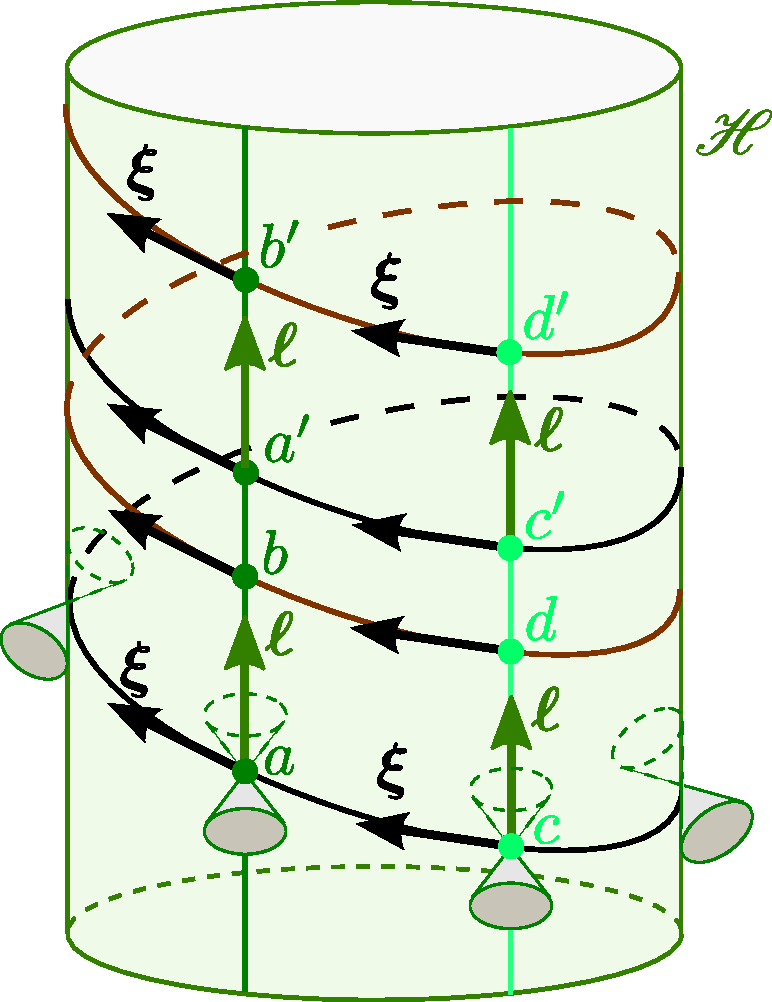
\includegraphics[height=0.4\textheight]{sta_rot_horizon_gen.pdf}
\qquad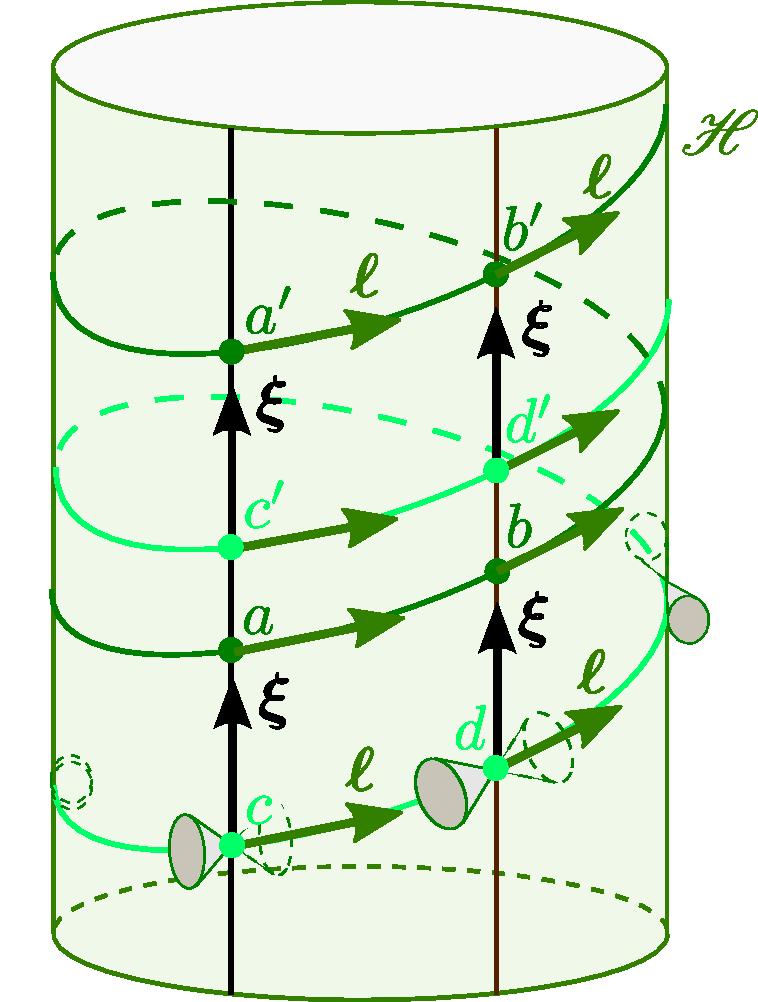
\includegraphics[height=0.4\textheight]{sta_rot_horizon_kil.pdf}}
\caption[]{\label{f:sta:rot_horizon} \footnotesize
Event horizon $\Hor$ with a stationary Killing vector field $\w{\xi}$ spacelike
on it:
\textbf{(a)} Representation with the null geodesic generators of $\Hor$ drawn as vertical
lines; two of them are actually depicted, in dark green and light green
respectively, with a null normal $\wl$ along them; besides,
two field lines of $\w{\xi}$
(orbits of the isometry group) are depicted, in black and brown
respectively.
\textbf{(b)} Representation with the field lines of $\w{\xi}$ as vertical lines.
The color code is the same as in (a) and
labelled points ($a$, $b$, etc.) help to identify
the two figures. A few light cones are drawn in each figure; note that $\w{\xi}$,
being spacelike,
is always outside of them,
while the null normal $\wl$ is always tangent to them. }
\end{figure}


\subsection{Spacelike stationary Killing field on $\Hor$: the strong rigidity theorem}
\label{s:sta:strong_rigidity}

When $\w{\xi}$ is spacelike on $\Hor$, it obviously cannot be collinear to
any null normal $\wl$ of $\Hor$.
Assuming that $\Hor$ has cross-sections of spherical topology, we observe
that, with respect to the null geodesic generators of $\Hor$, the field lines of $\w{\xi}$
form some helices, as depicted in Fig.~\ref{f:sta:rot_horizon}a. By reciprocity,
with respect to the field lines of $\w{\xi}$,
the null geodesic generators form some helices as well, as depicted in
Fig.~\ref{f:sta:rot_horizon}b):
observe that Fig.~\ref{f:sta:rot_horizon}b can be obtained from Fig.~\ref{f:sta:rot_horizon}a
by ``untwisting'' the field lines of $\w{\xi}$.

Since asymptotically the field lines of $\w{\xi}$ are worldlines of inertial observers,
Fig.~\ref{f:sta:rot_horizon}b leads us to say
(in loose terms at this stage) that the event horizon $\Hor$
``is rotating'', all the more that we have seen above that when the null
generators coincide with the field lines of $\w{\xi}$, the black hole is static, i.e. non-rotating.

Since the Killing field $\w{\xi}$ is not null on $\Hor$, we cannot say a priori
that $\Hor$ is a Killing horizon. However, modulo some additional hypotheses,
it turns out that this is the case, according to a famous result by
S.W.~Hawking\index{Hawking, S.W.} (1972)
\cite{Hawki72,HawkiE73}, known as the
\defin{strong rigidity theorem}\index{strong!rigidity theorem}\index{rigidity theorem!strong --}.
We give below a modern version of this theorem, due to Moncrief \& Isenberg
(2008) \cite{MoncrI08} (see also
Theorem~8.1 p.~470 of Choquet-Bruhat's textbook \cite{Choqu09})
\begin{prop}[strong rigidity theorem]
\label{p:sta:strong_rigidity_thm}
Let $(\M,\w{g})$ be a stationary spacetime of dimension $n\geq 4$ containing a black
hole of event horizon $\Hor$ such that the stationary Killing vector $\w{\xi}$
is spacelike on $\Hor$. If
\begin{itemize}
\item $\M$ and $\Hor$ are (real) analytic manifold
(cf. Remark~\ref{r:bas:analytic} in Sec.~\ref{s:bas:def_manif}),
with $\w{g}$ being an analytic field,
\item $\w{g}$ fulfills the vacuum Einstein equation
[Eq.~(\ref{e:fra:Einstein_eq}) with $\Lambda=0$ and $\w{T} = 0$],
\item $\Hor$ has a null geodesic generator that is incomplete,
\item $\Hor$ has compact cross-sections
\item $\w{\xi}$ is transverse to some cross-sections,
\end{itemize}
then the spacetime $(\M,\w{g})$ admits a second Killing vector field, $\w{\chi}$
say, such that
$\Hor$ is a Killing horizon with respect to $\w{\chi}$.
\end{prop}

\begin{hist}
The original version of the theorem established in 1972
by Stephen Hawking\index{Hawking, S.} \cite{Hawki72} was for a 4-dimensional
spacetime.
\end{hist}

The above theorem relies on the rather strong assumption that
the manifolds and fields are analytic.
On physical grounds,
it would be desirable to assume only \emph{smooth} manifolds and fields.
Recently, S.~Alexakis, A.D.~Ionescu and S.~Klainerman \cite{AlexaIK14} (2014)
have succeeded in proving the strong rigidity theorem without the analyticity
assumption, but only for slowly rotating black holes.

Since we have two Killing vectors, $\w{\xi}$ and $\w{\chi}$, we may
form any linear combination of them with constant coefficients
and still get a Killing vector. For instance, if $\Omega_H$ is a non-zero constant,
the vector field $\w{\eta}$ defined by
\be
    \w{\eta} = \frac{1}{\Omega_H} \left( \w{\chi} - \w{\xi} \right)
    \quad\iff\quad
    \w{\chi} = \w{\xi} + \Omega_H \w{\eta} ,
\ee
is a Killing vector field on $\M$.
One can show (see e.g. \cite{Chrus97} for a rigorous proof) that $\Omega_H$
and some constant rescaling of $\w{\chi}$
can be chosen so that $\w{\eta}$ is a spacelike vector field whose
field lines are closed, with $2\pi$-periodicity in terms of the parameter $\ph$
associated to $\w{\eta}$ (i.e. $\w{\eta} = \D/\D\ph$ along the field lines),
and such that $\w{\eta}$ vanishes on a timelike 2-dimensional surface, called
the \defin{rotation axis}\index{rotation!axis}.
It follows that
the isometry group whose generator is $\w{\eta}$ is the rotation group
$\mathrm{SO}(2)$. In other words, the spacetime $(\M,\w{g})$ is
\defin{axisymmetric}\index{axisymmetric!spacetime} in addition to being stationary.
The constant $\Omega_H$ is then called the
\defin{black hole rotation velocity}\index{black hole!rotation velocity}\index{rotation!velocity}.

By the very definition of stationarity, the Killing vector field $\w{\xi}$ is
timelike in the vicinity of $\scri^+$ and $\scri^-$. If $\w{\xi}$ is spacelike
on $\Hor$, as assumed in this section, by continuity it must be spacelike
in some part of the domain of outer communications $\langle\langle \M\rangle\rangle$
near $\Hor$. The simplest configuration is then when
$\w{\xi}$ is spacelike in some connected region $\mathscr{G}\subset \langle\langle \M\rangle\rangle$
around $\Hor$, null at the boundary of $\mathscr{G}$ and timelike outside $\mathscr{G}$
up to $\scri^+$ and $\scri^-$. The subset $\mathscr{G}$ is
called the \defin{ergoregion}\index{ergoregion} and its boundary $\E:=\partial\mathscr{G}$
the \defin{ergosphere}. We shall discuss it further in connection with
the Penrose process in Chap.~\ref{s:ker}.


%%%%%%%%%%%%%%%%%%%%%%%%%%%%%%%%%%%%%%%%%%%%%%%%%%%%%%%%%%%%%%%%%%%%%%%%%%%%%%%

\section{The no-hair theorem} \label{s:sta:no-hair}

\subsection{Israel uniqueness theorem for static black holes}

\begin{prop}[Israel uniqueness theorem\index{Israel uniqueness theorem}]
\label{p:sta:Israel_uniqueness_thm}
If $(\M,\w{g})$ is a $n$-dimensional static spacetime
containing a black hole, with $\w{g}$ solution of the vacuum Einstein
equation, then the domain of outer communications of $\M$ is isometric
to the domain of outer communications of a $n$-dimensional Schwarzschild spacetime\index{Schwarzschild!spacetime}.
\end{prop}
This theorem has been proved in 1967 by W.~Israel \cite{Israe67},
and improved latter by many authors, in particular by
P. Chru\'sciel \& G. Galloway (2010) \cite{ChrusG10}, who removed
the hypothesis of analyticity (cf. Remark~\ref{r:bas:analytic} in Sec.~\ref{s:bas:def_manif}).
A demonstration of Israel's theorem can be found in Sec.~8.2 of
Straumann's textbook \cite{Strau13}.

So basically, in dimension $n=4$, i.e. when the staticity theorem (Property~\ref{p:sta:staticity_thm}) applies,
all stationary vacuum black holes with the stationary Killing field $\w{\xi}$ null
on $\Hor$ are nothing but Schwarzschild black holes, which we will study in detail in Chaps.~\ref{s:sch} to~\ref{s:max}.

\subsection{The no-hair theorem}

In dimension $n=4$, one can go much further then just claiming that the
event horizon of a stationary black hole must be a Killing horizon (Sec.~\ref{s:sta:EH_KH}).
One has indeed the \defin{Carter-Robinson theorem}\index{Carter-Robinson theorem}
(Carter\index{Carter, B.} 1971 \cite{Carte71}, Robinson\index{Robinson, D.C.} 1975 \cite{Robin75}):
any stationary and axisymmetric 4-dimensional asymptotically flat
black hole spacetime $(\M,\w{g})$ that is
solution of the vacuum Einstein equation with a connected regular
event horizon $\Hor$ and no closed timelike curve outside it
has a domain of outer communications that is isometric
to the domain of outer communications of the Kerr spacetime.

\begin{remark}
In their original works, Carter and Robinson assumed that $\Hor$ is a
\emph{non-degenerate}
Killing horizon, i.e. that the non-affinity coefficient $\kappa$ associated
with the Killing vector $\w{\chi}$ is non-zero (cf. Sec.~\ref{s:neh:classif_KH}). However, this non-degeneracy
hypothesis can be released \cite{ChrusN10} (see \cite{ChrusLH12} for an
extended discussion).
\end{remark}

\begin{remark}
The causality condition (absence of closed timelike curves in the black
hole exterior), which is one of the assumptions of Carter's theorem
(cf. \cite{Carte99} for a discussion), does not appear in Israel's theorem
(Property~\ref{p:sta:Israel_uniqueness_thm}) because a static spacetime, which by definition
has hypersurface-orthogonal timelike curves,
cannot contain any closed timelike curve.
\end{remark}

By combining the staticity, Israel, strong rigidity and Carter-Robinson theorems,
one arrives at the famous
\begin{prop}[no-hair theorem\index{no-hair theorem}]
Any spacetime $(\M,\w{g})$ that
\begin{itemize}
\item is 4-dimensional
\item is asymptotically flat
\item is stationary
\item is a solution of the vacuum Einstein equation
\item contains a black hole with a connected regular horizon
\item does not contain any closed timelike curve in the domain of outer
communications
\item is analytic
\end{itemize}
has a domain of outer communications that is isometric
to the domain of outer communications of the Kerr spacetime.
\end{prop}

See Ref.~\cite{IonesK15} for a review.

\begin{hist}
See the historical account by Carter \cite{Carte99}.
\end{hist}
